\def\year{2019}\relax
\documentclass[letterpaper]{article} % DO NOT CHANGE THIS
\usepackage{aaai19}  % DO NOT CHANGE THIS
\usepackage{times}  % DO NOT CHANGE THIS
\usepackage{helvet} % DO NOT CHANGE THIS
\usepackage{courier}  % DO NOT CHANGE THIS
\usepackage[hyphens]{url}  % DO NOT CHANGE THIS
\usepackage{graphicx} % DO NOT CHANGE THIS
\urlstyle{rm} % DO NOT CHANGE THIS
\def\UrlFont{\rm}  % DO NOT CHANGE THIS
\usepackage{graphicx}  % DO NOT CHANGE THIS
\frenchspacing  % DO NOT CHANGE THIS
\setlength{\pdfpagewidth}{8.5in}  % DO NOT CHANGE THIS
\setlength{\pdfpageheight}{11in}  % DO NOT CHANGE THIS
\usepackage{amsmath}
\graphicspath{{images/}}
\nocopyright
\usepackage{array}
\usepackage{caption}
\usepackage{xcolor}
\usepackage[outputdir=output]{minted}
\usepackage{changepage}
%PDF Info Is REQUIRED.
% For /Author, add all authors within the parentheses, separated by commas. No accents or commands.
% For /Title, add Title in Mixed Case. No accents or commands. Retain the parentheses.
\pdfinfo{
/Title (Decision Trees)
/Author (Mark Wesley Harris)
} %Leave this	
% /Title ()
% Put your actual complete title (no codes, scripts, shortcuts, or LaTeX commands) within the parentheses in mixed case
% Leave the space between \Title and the beginning parenthesis alone
% /Author ()
% Put your actual complete list of authors (no codes, scripts, shortcuts, or LaTeX commands) within the parentheses in mixed case. 
% Each author should be only by a comma. If the name contains accents, remove them. If there are any LaTeX commands, 
% remove them. 

% DISALLOWED PACKAGES
% \usepackage{authblk} -- This package is specifically forbidden
% \usepackage{balance} -- This package is specifically forbidden
% \usepackage{caption} -- This package is specifically forbidden
% \usepackage{color (if used in text)
% \usepackage{CJK} -- This package is specifically forbidden
% \usepackage{float} -- This package is specifically forbidden
% \usepackage{flushend} -- This package is specifically forbidden
% \usepackage{fontenc} -- This package is specifically forbidden
% \usepackage{fullpage} -- This package is specifically forbidden
% \usepackage{geometry} -- This package is specifically forbidden
% \usepackage{grffile} -- This package is specifically forbidden
% \usepackage{hyperref} -- This package is specifically forbidden
% \usepackage{navigator} -- This package is specifically forbidden
% (or any other package that embeds links such as navigator or hyperref)
% \indentfirst} -- This package is specifically forbidden
% \layout} -- This package is specifically forbidden
% \multicol} -- This package is specifically forbidden
% \nameref} -- This package is specifically forbidden
% \natbib} -- This package is specifically forbidden -- use the following workaround:
% \usepackage{savetrees} -- This package is specifically forbidden
% \usepackage{setspace} -- This package is specifically forbidden
% \usepackage{stfloats} -- This package is specifically forbidden
% \usepackage{tabu} -- This package is specifically forbidden
% \usepackage{titlesec} -- This package is specifically forbidden
% \usepackage{tocbibind} -- This package is specifically forbidden
% \usepackage{ulem} -- This package is specifically forbidden
% \usepackage{wrapfig} -- This package is specifically forbidden
% DISALLOWED COMMANDS
% \nocopyright -- Your paper will not be published if you use this command
% \addtolength -- This command may not be used
% \balance -- This command may not be used
% \baselinestretch -- Your paper will not be published if you use this command
% \clearpage -- No page breaks of any kind may be used for the final version of your paper
% \columnsep -- This command may not be used
% \newpage -- No page breaks of any kind may be used for the final version of your paper
% \pagebreak -- No page breaks of any kind may be used for the final version of your paperr
% \pagestyle -- This command may not be used
% \tiny -- This is not an acceptable font size.
% \vspace{- -- No negative value may be used in proximity of a caption, figure, table, section, subsection, subsubsection, or reference
% \vskip{- -- No negative value may be used to alter spacing above or below a caption, figure, table, section, subsection, subsubsection, or reference

\setcounter{secnumdepth}{0} %May be changed to 1 or 2 if section numbers are desired.

% The file aaai19.sty is the style file for AAAI Press 
% proceedings, working notes, and technical reports.
%
\setlength\titlebox{2.5in} % If your paper contains an overfull \vbox too high warning at the beginning of the document, use this
% command to correct it. You may not alter the value below 2.5 in
\title{Decision Trees}
%Your title must be in mixed case, not sentence case. 
% That means all verbs (including short verbs like be, is, using,and go), 
% nouns, adverbs, adjectives should be capitalized, including both words in hyphenated terms, while
% articles, conjunctions, and prepositions are lower case unless they
% directly follow a colon or long dash
\author{Mark Wesley Harris\\ % All authors must be in the same font size and format. Use \Large and \textbf to achieve this result when breaking a line
% If you have multiple authors and multiple affiliations
% use superscripts in text and roman font to identify them. For example, Sunil Issar,\textsuperscript{\rm 2} J. Scott Penberthy\textsuperscript{\rm 3} George Ferguson,\textsuperscript{\rm 4} Hans Guesgen\textsuperscript{\rm 5}. Note that the comma should be placed BEFORE the superscript for optimum readability
University of Colorado Colorado Springs\\
wharris2@uccs.edu % email address must be in roman text type, not monospace or sans serif
}
\begin{document}

\maketitle

\section{Introduction}
Linear regression is not always suitable for classification.
After all, it is not guaranteed that any dataset will fit a linear regression problem.
Research has shown that in these situations it may be useful instead to use a decision tree as a classifier.
Boosting trees are a type of decision tree that focus on converging to an answer iteratively,
much like Stochastic Gradient Descent.
There have been many boosting algorithms, including Discrete and Real AdaBoost --
an additive tree building algorithm with an exponential loss function \cite{additive}.
The algorithm used for boosting in general is called gradient boosting,
where any loss function and tree schema can be used.
It is the discussion and implementation of this
algorithm which we focus on in this paper.

\subsection{Boosting}
Boosting trees are additive, meaning they are built to correct the error from
the previous tree in a sequence.
An ensemble of boosting trees are added together in order to classify an input vector.
In this way
``\dots boosting bears a resemblance to bagging and other
committee-based approaches,'' however boosting is notably different
\cite{elements}.
The additive model of boosting trees is expressed by Equation
\ref{eq:boost} \cite{elements}.

\begin{equation}
\label{eq:boost}
f_M(x) = \sum_{m = 1}^{M}\beta_mb(x;\gamma_m)
\end{equation}

Weak-learners are used for the implementation of the boosting algorithm.
A weak-learner is is a small tree that classifies
correctly with a probability greater than chance
For binary decisions this means $>50\%$ of the time.
There is research to suggest that trees of sizes $4 \leq J \leq 8$ perform best,
although they found there is
``\dots no significant improvement over using $J \simeq 6$'' \cite{elements}.
Weak-learners are faster to build and evaluate than strong learners,
making them perfect for boosting trees.
A single weak-learner is not very powerful in the context of classification;
by adding together hundreds of weak-learners however, we can find an answer
to the problem with increased predictability given new data.

\subsection{Gradient Tree Boosting}
%Question 3(1)
In Gradient Tree Boosting, the goal is to minimize the gradient of function
$f(x)$.
To simplify the gradient calculation, we use the squared loss equation,
$L(y,f(x)) = \frac{1}{2}(y - f(x))^2$,
where $y$ is the true value and $f(x)$ is the prediction.
Gradient boosting uses the same concepts as gradient descent;
each generation we find the ``step'' to take that will minimize the gradient.
%This step is shown by line 2(a) of the Gradient Tree Boosting algorithm,
%shown below:
For reference, the Gradient Tree Boosting algorith is produced below.
\bigskip
\begin{adjustwidth}{1em}{1em}
\begin{enumerate}
\item Initialize $f_0(x) = argmin_{\gamma}\sum_{i=1}^NL(y_i,\gamma)$.
\item For $m = 1$ to $M$:
\begin{adjustwidth}{1em}{0em}
\begin{enumerate}
\item For $i = 1,2,\dots,N$ compute
$$
r_{im} =
-\left[
\frac{\partial L(y_i,f(x_i))}{\partial f(x_i)}
\right]_{f=f_{m - 1}} \text{.}
$$
\item Fit a regression tree to the targets $r_{im}$ giving terminal regions
$R_{jm}, j = 1,2,\dots,J_m$.
\item For $j = 1,2,\dots,J_m$ compute
$$
\gamma_{jm} = argmin_{y}\sum_{x_i\in R_{jm}}L(y_i,f_{m - 1}(x_i) + \gamma) \text{.}
$$
\item Update $f_m(x) = f_{m - 1}(x) + \sum_{j=1}^{J_m}\gamma_{jm}I(x\in R_{jm})$.
\end{enumerate}
\end{adjustwidth}
\item Output $\hat{f}(x) = f_M(x)$
\end{enumerate}
\end{adjustwidth}
\bigskip
%\begin{figure}[htbp]
%\centerline{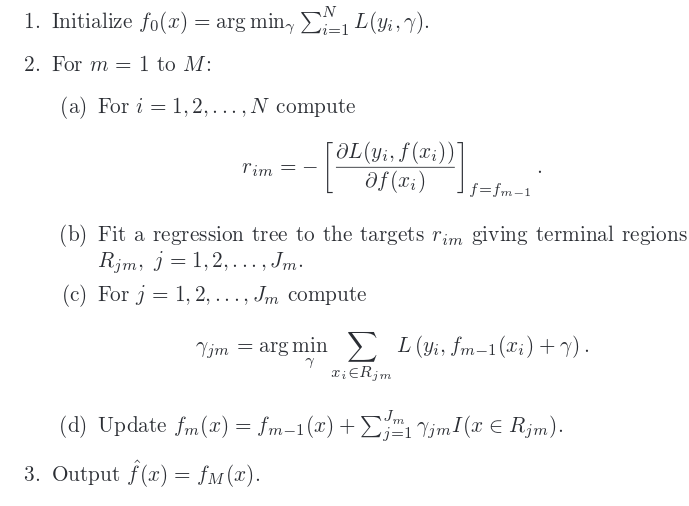
\includegraphics[width=8cm]{grad_tree_boosting.png}}
%\caption{Gradient Tree Boosting Algorithm
%\cite{elements}.}
%\label{fig:grad_tree_boosting}
%\end{figure}

%There are two important calcuations here,
%$r_{im}$ and $\gamma_{jm}$.
%The steps of the algorithm are broken down by line below.
Line 1 is the initialization phase that occurs before the main loop.
$f_0$ classifies all input as the average of the real values, $y_i$.
This serves to create a prediction represented by a horizontal
hyperplane at $y = avg(y)$ for all $x_i$ attributes.

The calculation of $
r_{im} =
-\left[
\frac{\partial L(y_i,f(x_i))}{\partial f(x_i)}
\right]_{f=f_{m - 1}}
$
uses the gradient, $\nabla L$, to create a split in the data to evaluate.
For the squared loss being used, the gradient simplifies to
$\nabla L = f_{m-1}(x_i) - y_i$,
which is to say the difference between the real value
and corresponding psuedo-residue.
Lines 2(b) through 2(c) are then used to find the smallest gradient
for the calculation of the next weak-learner on line 2(d).

Trees $m = 1,2,\dots,M$ do not work in the same way as the initial one, $f_0$.
They instead focus on correcting the mistakes of the previous weak-learner
in the series.
Thus the new tree, $f_m$, is a classifier from the previous tree's psuedo-residues.
For the first case, it is simply $f_1 = y_i - f_{0}(x_i)$.
The rest of the trees follow the pattern
$f_m = f_{m-2}(x_i) - f_{m-1}(x_i)$.
For our implementation we also introduced
a learning parameter, $\lambda$, to curb the effects
of each weak-learner and prevent over-training.
Using the additive property of gradient boosting,
we can predict an output for a given input vector, $x$,
with the formula below.

$$\hat{f}(x) = f_0(x) + \sum_{i = 1}^M\lambda f_{i}(x)$$

%\subsection{Splitting}
In general, splitting for Regression Trees can be accomplished by
analyzing the variance of each split candidate for each attribute.
The formula for splitting off of variance is given in Equation \ref{eq:var}
\cite{kalita}.

\begin{equation}
\label{eq:var}
\Delta(D,f_j) = Var(D) - \sum_{i=1}^{nv(f)_j}\frac{|D_{f_i}|}{|D|}Var(D_{f_i})
\end{equation}

Gradient boosting does not use variance, however. Instead, we split on the value of the gradient.
By the nature of gradient descent, the Mean Squared Error (MSE) will decrease at each iteration.
This effect is shown in the trends of Figure \ref{fig:mse_evaluation}.

\section{Implementation}
%Question 1(0)
The pseudocode for Classification and Regression Trees (CART) is given in Figure \ref{fig:cart}.
The CART model is used in a general sense for creating trees, boosting and otherwise
\cite{cart}.
As discussed above, the criteria for creating a tree with gradient boosting
is a split on the smallest gradient given all split cases of the attributes.
The format for creating leaf nodes was also taken from the CART source,
with the rule that ``an instance goes left if $condition$, and goes right otherwise
where the $condition$ is expressed as `attribute $X_i \leq C$' for continuous attributes'' \cite{top10}.

\begin{figure}[htbp]
\centerline{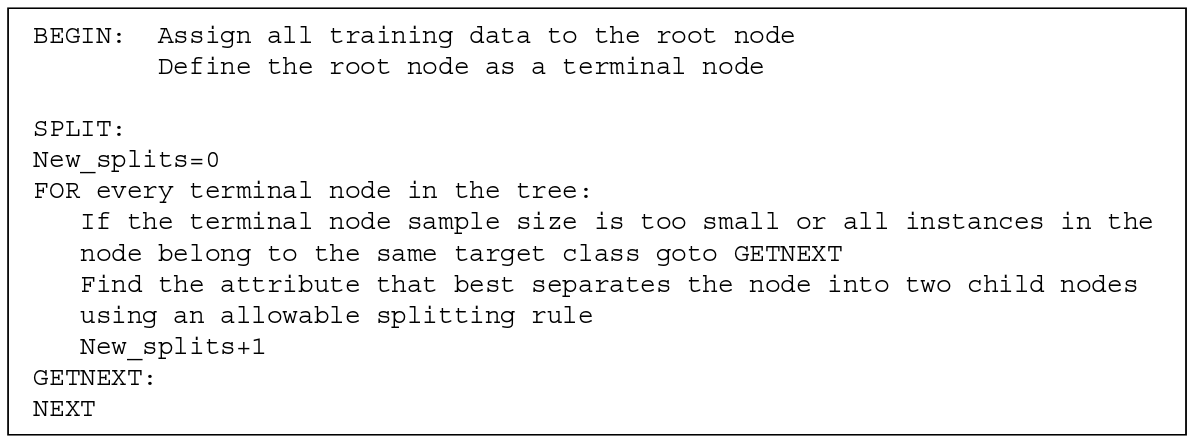
\includegraphics[width=8cm]{cart.png}}
\caption{Pseudocode for CART
\cite{top10}.}
\label{fig:cart}
\end{figure}

\subsection{Stumping}
Two-leaf stumps were used as the trees for the gradient boosting algorithm.
These stumps are extreemely weak-learners in the sense that they have one root node
and two leaf nodes.
Stumps often perform ``\dots worse than chance on the whole dataset,
but by using the weights to sort out when that classifier should be used\dots
the overall output of stumping can be very successful'' \cite{machine_learning}. %-- page 273
The ``weights'' in the Gradient Tree Boosting algorithm are a combination of
the learning parameter and corrections made via classification of the psuedo-residues.
Further weighting can be applied per tree in a more particular
fashion, however this and other optimizations are not explored here.

\subsection{Implementation Details}
Implementation for the Gradient Tree Boosting algorithm was performed
in Python.
First an implementation was written for creating a stump
given a vector of float values. In order to create the stump,
the best split of $k$ splits is evaluated.
A value of $k = 10$ was used for testing, which implies the vectors were
split into deciles. In general, varying $k$ past 10 did not drastically improve perfomance.
The averge of the boundaries between split candidates were tested
for the smallest gradient by using the results of the split.
%, as expressed
%in Equation \ref{eq:split} below.
%\begin{equation}
%\label{eq:split}
%\sum_{x_i\in R_{jm}}avg(y_{i}) - p_{i}
%\end{equation}
The final information stored within each stump
(implemented as a Python dictionary) is outlined below:
\bigskip
\begin{itemize}
\item ``attribute'' -- the name of the attribute chosen for splitting.
\item ``value'' -- the value on which the attribute is split.
\item ``gradient'' -- the gradient ($\nabla L$) of the chosen split,
which is ensured to be the lowest gradient among the splits for the given column.
\item ``left'' -- the left leaf value, i.e. when $x_i <= value$.
\item ``right'' -- the right leaf value, i.e. when $x_i > value$.
\end{itemize}
\bigskip
Since finding a stump invloves evaluating and splitting data,
helper functions were written for ease of code manipulation.
Finally, the main loop was constructed where stumps are evaluated.
One of the nuances of the implementation was deciding the
stopping conditions of the program --
it was noted that at times corrections to the pseudo-residues became so
incredibly small that no noticable change occured in the output stump.
This was not only a time-sink for the program, but also a distraction
from corrections to the other attributes being evaluated.
In order to create a more balanced approach, a variable $\varepsilon = 0.01$
was used to cap the processing of attributes.
Thus, the main loop exits when either the tree count $M = 150$ is reached
or when all attributes can no longer be updated for better results in the
output.

\subsection{Evaluation}
The Combined Cycle Power Plant dataset
found in the UCI Machine Learning Repository was used to test the implementations.
The dataset represents a distribution for energy output ($PE$),
which is based on the features of
average temperature ($AT$),
exhaust vacuum ($V$),
ambient pressure ($AP$),
and relative humidity ($RH$).
Thus, the optimization problem presented is to predict $PE$ given
values for $AT$, $V$, $AP$, and $RH$.

Implementations using Python and R libraries were created
to serve as comparisons of the non-library approach.
To evaluate all 3 implementations, the CCPP dataset was split into 75\% training data and 25\% test data
after shuffling. Thus, the models are not evaulated on how well they fit the
training data, but how well they can make predictions based on the test data.
All programs were run multiple times in sequence to ensure the results of the prediction were
independent of the separation of the dataset.

\section{Results}
Figure \ref{fig:mse_evaluation} shows the implementation of the
Gradient Tree Boosting algorithm for different sizes of learning parameter,
$\lambda$. Table \ref{tbl:contrast} demonstrates the ability of the learning
parameter to affect the algorithm output, by contrasting
final mean squared error (MSE), tree count,
and the required time for the program to run.
Table \ref{tbl:goodness} compares the goodness of the library implementations
and the implementation from scratch.
Not only are the $R^2$ values much better for the library implementations,
they also run much faster than the program implemented from scratch.
Specifically, the Python library performed exceptionally faster than the R
library. That is not to say that the R library
performed poorly, it may simply be a result of an inexperience with the R
programming language or unoptimized input training parameters.

\begin{table}[t]
\begin{centering}
\bgroup
\def\arraystretch{1.5}
\begin{tabular}{| m{0.085\textwidth} || m{0.095\textwidth} | m{0.095\textwidth}| m{0.095\textwidth}|} 
\hline
$\lambda$ & MSE & Tree Count & Relative Time \\ 
\hline
\hline
$\lambda = 0.25$ & 153.5684 & 150 & Longest \\
\hline
$\lambda = 0.50$ & 132.6641 & 103 & Middle \\
\hline
$\lambda = 0.75$ & 161.7242 & 92 & Shortest \\
\hline
\end{tabular}
\caption{Results of Non-Library implementation depending on learning parameter, $\lambda$.}
\label{tbl:contrast}
\egroup
\end{centering}
\end{table}

\begin{table}[t]
\begin{centering}
\bgroup
\def\arraystretch{1.5}
\begin{tabular}{| m{0.10\textwidth} | m{0.15\textwidth} | m{0.15\textwidth}|} 
\hline
Method & $R^2$ & MSE \\ 
\hline
\hline
Non-Library ($\lambda = 0.5$) & 0.5548111 & 132.6641026 \\
\hline
R-Library & 0.9632228 & 3.290562 \\
\hline
Python-Library & 0.9446135 & 16.8201 \\
\hline
\end{tabular}
\caption{Evaluation for the goodness of fit.}
\label{tbl:goodness}
\egroup
\end{centering}
\end{table}

The results of the non-library implementation are poor
compared to both the library implementations. This result could be depenent upon several factors.
Using stumps incompliant with the $J \simeq 6$ rule could have brought performance down.
The tuning of hyperparameters could also play a role in the quality of predictions \cite{elements}.
Finally, the algorithm could not build as many trees nor as quickly as the library implementations,
which used an ensemble of 10,000 trees to make their prediction.
Thus, the non-library implementation was bounded by both processing power and time.
The general trend in MSE, however, implies that
our implementation could see as good results as the library implementations after optimization
of the above caveats.

\section{Conclusion}
Implementing regression trees is no simple task.
Even the code for creating a simple stump was complicated,
and involved trial and error within the implementation space.
The library implementations ultimately proved to be much better
than the program written from scratch.
However, comparing our results to a single weak-learner,
it is clear that the ensemble approach employed by
gradient boosting is much better than the results of a single weak-learner.
Since the CCPP dataset invloves only 4 attributes,
it would also be difficult to make a strong learner perform better than
an ensemble of gradient boosting trees.

It is noteworthy to compare the libraries to the other regression
approaches evaluated in the previous assignment on regression -- both the Python and R library implementations
had better $R^2$ values than the regression fits found previously.
Therefore, the gradient boosting tree algorithm proved to be a better model
to use for classifying the CCPP data.

\begin{figure}[htbp]
\centerline{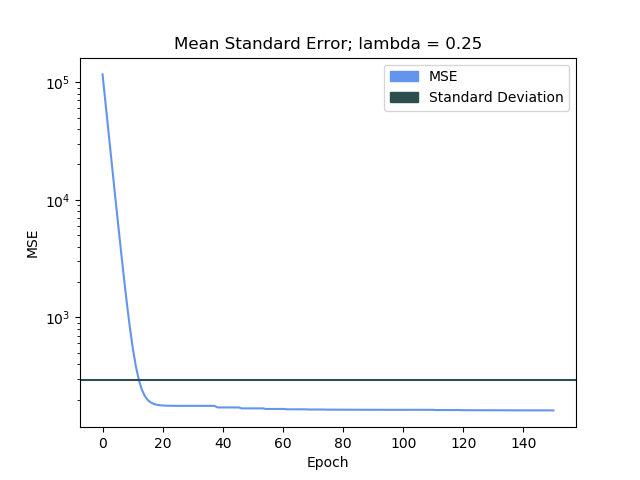
\includegraphics[width=8cm]{trees_25.png}}
\centerline{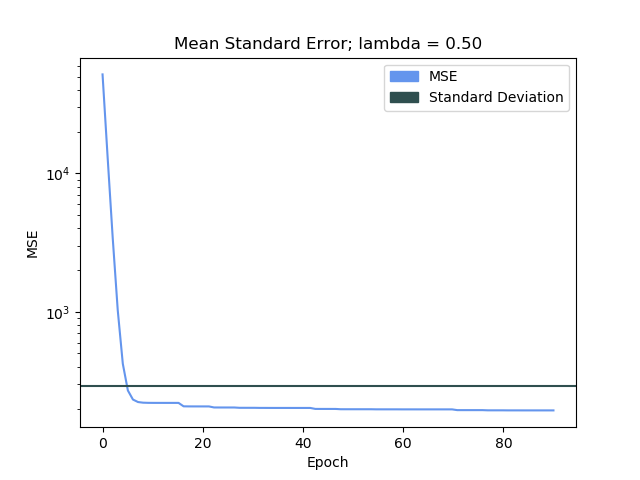
\includegraphics[width=8cm]{trees_50.png}}
\centerline{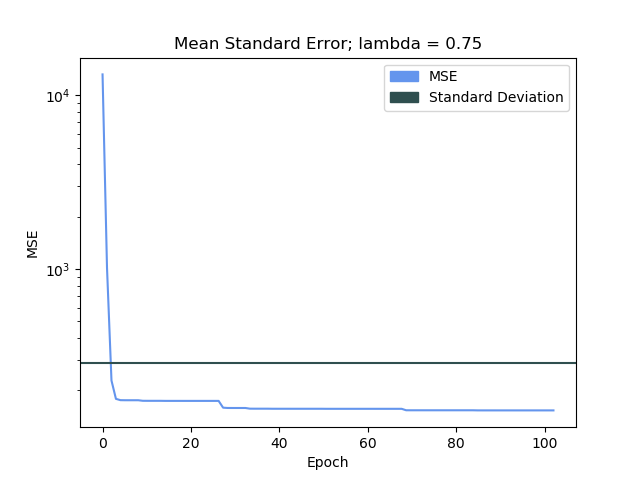
\includegraphics[width=8cm]{trees_75.png}}
\caption{Mean Squared Error of Non-Library implementation for variable epochs using learning parameter
$\lambda = 0.25,0.50,0.75$ respectively.
The standard deviation for the MSE is shown in each graph as a dark grey line.
Final MSE values are shown in Table \ref{tbl:contrast}.}
\label{fig:mse_evaluation}
\end{figure}
%\begin{figure*}[tbp]
%\centerline{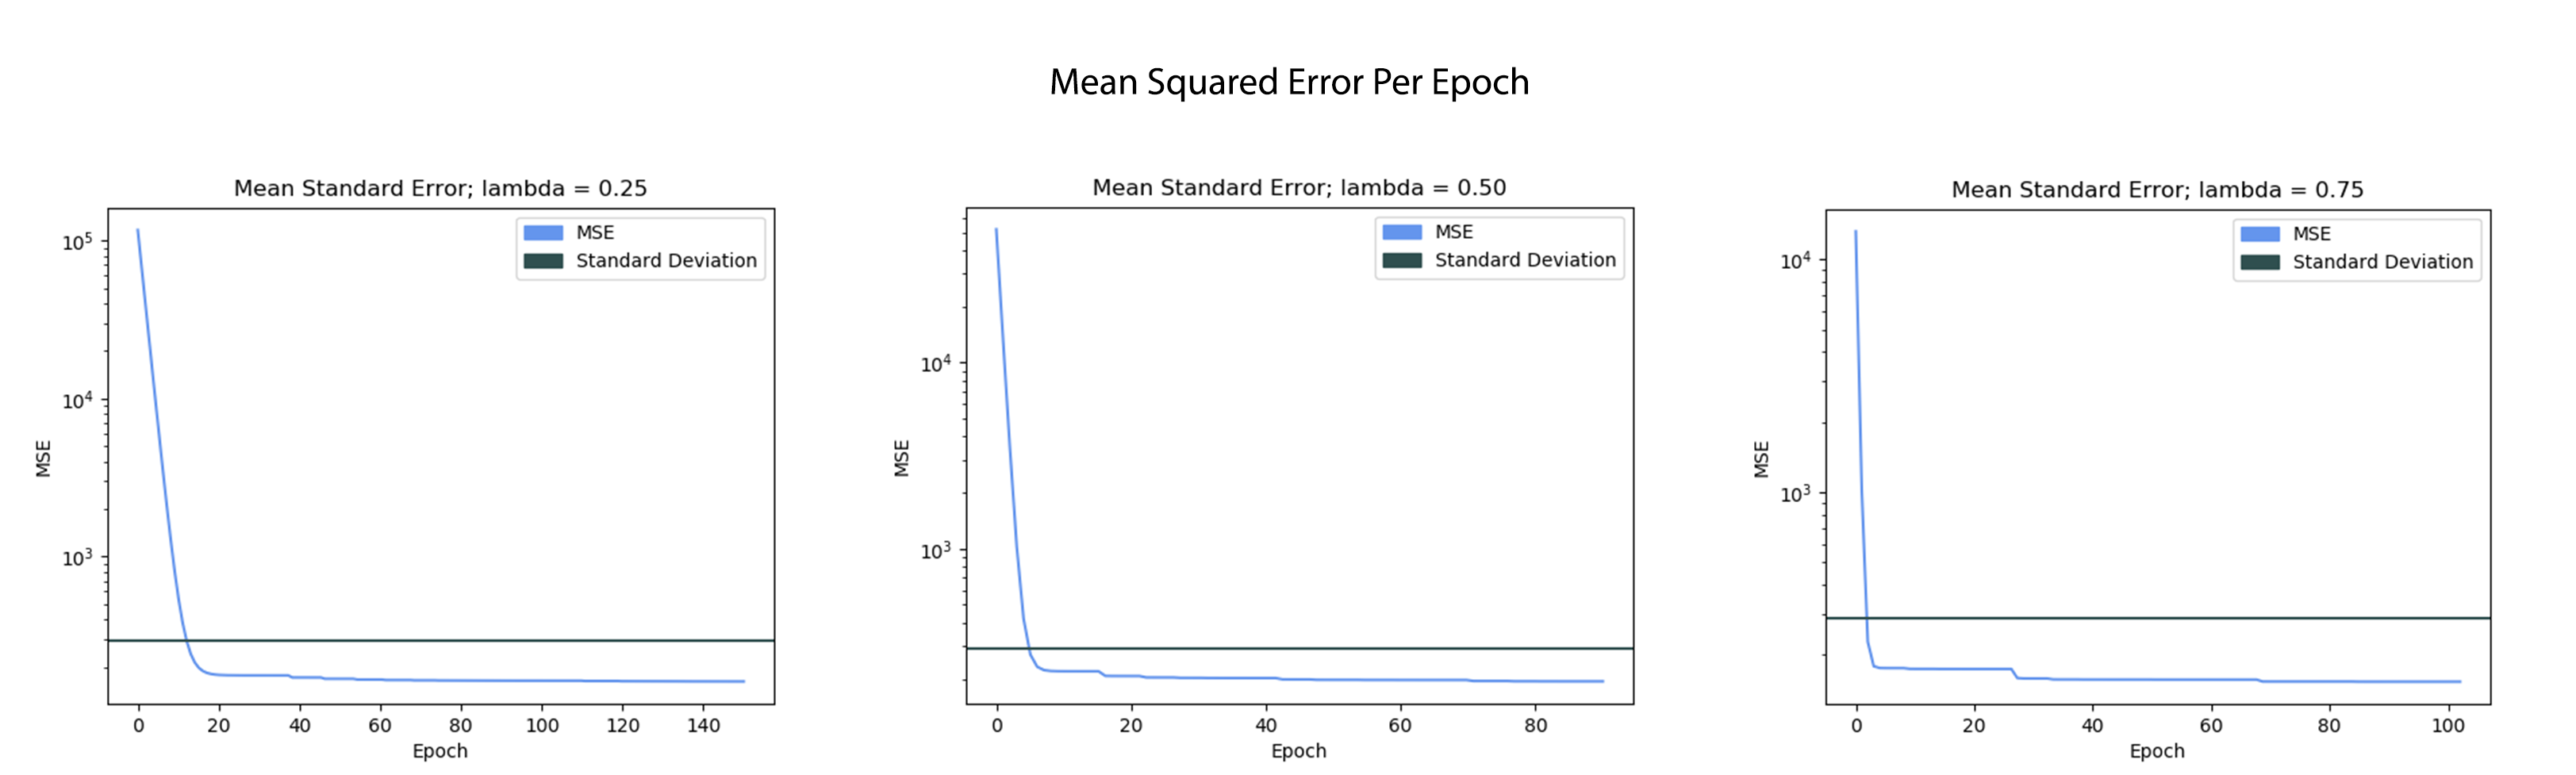
\includegraphics[width=\textwidth]{mse_evaluation.png}}
%\caption{Mean squared error for variable epochs using learning parameter
%$\lambda = 0.25,0.50,0.75$ respectively.
%The standard deviation for the MSE is shown in each graph as a dark grey line.
%Means and final MSE values are shown in Table \ref{tbl:contrast}.}
%\label{fig:mse_evaluation}
%\end{figure*}

\bibliography{report}
\bibliographystyle{aaai}

\begin{figure}[htbp]
\centerline{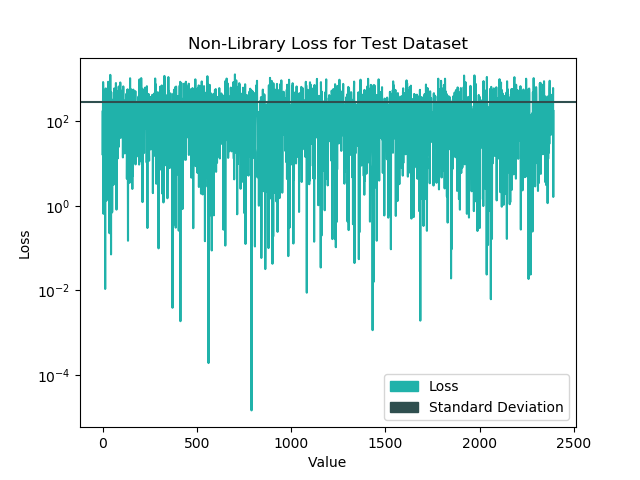
\includegraphics[width=8cm]{non_lib_loss.png}}
\caption{Loss for the Non-Library implementation on the test set.}
\label{fig:non-lib}
\end{figure}

\begin{figure}[htbp]
\centerline{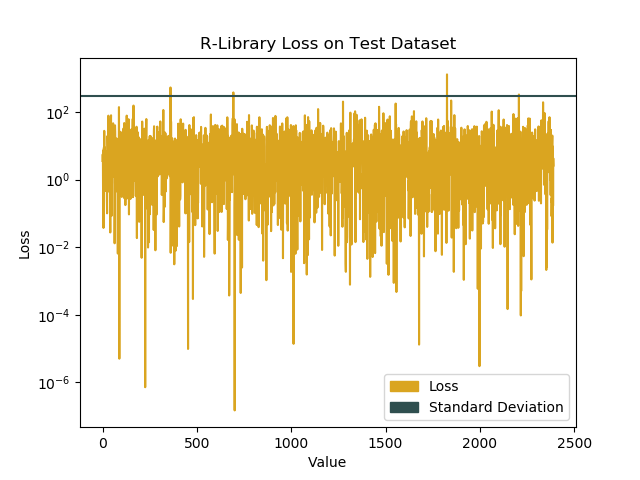
\includegraphics[width=8cm]{r_lib_loss.png}}
\caption{Loss for the R-Library implementation on the test set.}
\label{fig:r-lib}
\end{figure}

\begin{figure}[htbp]
\centerline{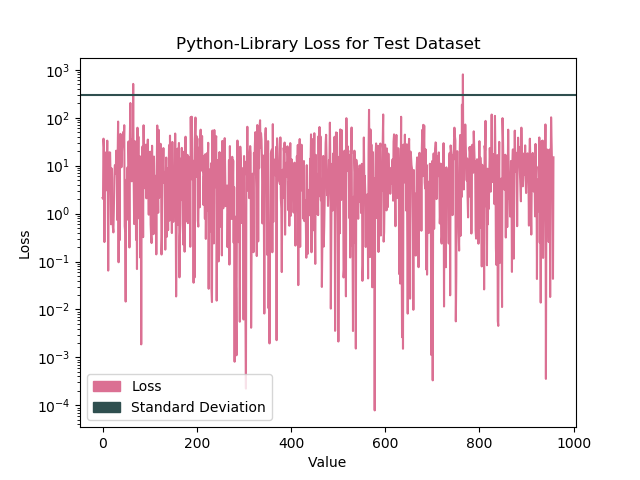
\includegraphics[width=8cm]{python_lib_loss.png}}
\caption{Loss for the Python-Library implementation on the test set.}
\label{fig:python-lib}
\end{figure}

\onecolumn

\pagebreak

\begin{center}
\section*{Appendix}
\label{app:b}
\end{center}

\bigskip

\footnotesize{
\begin{minted}{python}
# tree.py
import math as math
import pandas as pd
import numpy as np
import utilities
import sys

# Define method for splitting y on value of x.
def split_col(x, y, val):
    l_set, r_set = [], []
    count = 0
    
    # Add x to l_set or r_set, depending on val.
    #for data in dataset.loc[:,col]
    for index in range(1, len(x)):
        if x[index] <= val:
            l_set.append(y[index])
        else:
            r_set.append(y[index])

    return l_set, r_set

# Define method for splitting dataset on value and column.
def split_dataset(dataset, x, val):
    l_set, r_set = [], []
    
    # Add rows to l_set or r_set, depending on val.
    for index, data in dataset.iterrows():
        if x[index] <= val:
            l_set.append(data.values.tolist())
        else:
            r_set.append(data.values.tolist())

    return np.array(l_set), np.array(r_set)

# Define method for obtaining min gradient for a list of values.
def min_gradient(dataset, x, k):
    # Initialize variables.
    val = 0
    grad = math.inf
    sections = np.array_split(np.sort(x), min(k + 1, len(x)))

    # Use k = len(col = dataset[:,*]), i.e. check each value.
    for i in range(1, len(sections)):
        curr_val = (sections[i][0] + sections[i - 1][len(sections[i - 1]) - 1]) / 2

        # Split dataset based on sample value.
        l_set, r_set = split_dataset(dataset, x, curr_val)
        l_grad = np.average(l_set[:,4]) - np.average(l_set[:,5])
        r_grad = np.average(r_set[:,4]) - np.average(r_set[:,5])
        curr_grad = l_grad + r_grad

        # Store sample if current gradient is lowest.
        if curr_grad < grad:
            val = curr_val
            grad = curr_grad

        sys.stdout.write('\r    [%d/%d][%d] : %f, %f' % (i, k, len(x) - 1, val, grad))

    print('\n')
    return val, grad

# Define method for creating a stump based off an input vector, x.
def create_stump(dataset, name):
    print('\n... Evaluating Column ' + str(name))
    x = dataset[name].values.tolist()
    y = dataset.iloc[:,4].values
    p = dataset.iloc[:,5].values

    # Find split and obtain leaf node values.
    val, grad = min_gradient(dataset, x, 10)
    l_set, r_set = split_col(x, p, val)
    left = np.average(l_set)
    right = np.average(r_set)
    
    epsilon = 0.01
    if abs(left) < epsilon or abs(right) < epsilon:
        print('%s is not applicable!' % (name))
        grad = math.inf

    # Store stump as dictionary of averages.
    stump = {
        'attribute' : name,
        'value' : val,
        'gradient' : grad,
        'left' : left,
        'right' : right
    }

    return stump
    

# Define method for creating the first stump based off variance of the dataset.
def stump_from_dataset(dataset):
    # Intialize variables.
    stump = {}
    var, col, val = 0, 0, 0
    cols = dataset.columns.get_values()
    y = dataset.iloc[:,4].values
    p = dataset.iloc[:,5].values

    # Find which variable to split on, skipping the final y column.
    for i in range(len(cols) - 2):
        # Create stump off of current column.
        curr_stump = create_stump(dataset, cols[i])

        # Test if stump is a better classifier.
        if stump == {} or curr_stump['gradient'] < stump['gradient']:
            stump = curr_stump

    return stump

# Define method for creating another stump (i.e. weak classifier).
def next_stump(dataset, stumps):
    # Initialize helper variables.
    cols = dataset.columns.get_values()
    y = dataset.iloc[:,4].values
    stump = {}
    rim = []

    # ln 1: Special case, average all y(i) values for each x(i).
    #       The feature to use as root is chosen based off max change
    #       in variance.
    if len(stumps) == 0:
        # Overwrite stump value with average.
        init_subset = dataset
        init_subset['PR'] = np.average(y)
        stump = stump_from_dataset(init_subset)

    # Else build off of previous stump using gradient boosting.
    else:
        # ln 2(a): Find r(i)(m) for x(i) in data columns.
        for index, data in dataset.iterrows():
            rim.append(data['PE'] - utilities.evaluate(stumps, data))

        # ln 2(b): Fit a regression tree to targets r.
        rim_subset = dataset
        rim_subset['PR'] = rim
        stump = stump_from_dataset(rim_subset)

    stumps.append(stump)
    print(stump)
    print(utilities.mse(dataset, stumps))

    return stumps

# Load dataset.
dataset = utilities.import_CCPP(False)
length = len(dataset.iloc[:,1])
ratio = int(length * 0.75)
train_dataset = dataset.iloc[0:ratio]
test_dataset = dataset.iloc[ratio:]

# Initialize list of classifiers and roots.
stumps = []
losses = []
m = 150

for i in range (1, m + 1):
    print("Step %d of %d\n" % (i, m))
    stumps = next_stump(train_dataset, stumps)
    losses.append(utilities.mse(train_dataset, stumps))
    # Save trees to a file.
    f = open("trees_%d.txt" % (m), "a+")
    f.write("%s:%f:%f:%f:%f\n" % (stumps[-1]['attribute'], stumps[-1]['value'],
                                  stumps[-1]['left'], stumps[-1]['right'], losses[-1]))
    f.close()
    
    # Check stopping condition(s).
    if stumps[-1]['gradient'] == math.inf:
        m = i
        break

utilities.plot_loss(m, losses, train_dataset, 'Mean Standard Error; lambda = 0.50',
                    'cornflowerblue')

test_losses = []
y_test = test_dataset.iloc[:,4].values.tolist()
for index, data in test_dataset.iterrows():
    test_losses.append((data['PE'] - utilities.evaluate(stumps, data)) ** 2)

utilities.plot_test(test_losses, y_test, 'Non-Library Loss for Test Dataset', 'lightseagreen')
utilities.stats(test_dataset, stumps, 'Gradient Boosting Tree Algorithm')
\end{minted}
\bigskip
\begin{minted}{python}
# library.py
# Modeled off of "Gradient Boosting regression" on SciKit Learn (Library)
# Source: https://scikit-learn.org/stable/auto_examples/ensemble/plot_gradient_
          boosting_regression.html

import pandas as pd
import numpy as np
import matplotlib.pyplot as plt
import matplotlib.patches as mpatches
import utilities

from sklearn import ensemble
from sklearn.metrics import mean_squared_error

# Definition for Squared Sum of Errors.
def SSE(y_real, y_pred):
    sse = 0
    for index in range(len(y_real)):
        sse += (y_real[index] - y_pred[index]) ** 2

    return sse

# Definition for Squared Sum of Total Error.
def SST(y_real):
    sst = 0
    y_mean = np.mean(y_real)
    for index in range(len(y_real)):
        sst += (y_real[index] - y_mean) ** 2

    return sst

# Definition for R^2.
def R_squared(y_real, y_pred):
    return (1 - SSE(y_real, y_pred) / SST(y_real))

# Load dataset.
dataset = utilities.import_CCPP(False)
x = dataset.iloc[:,0:4]
y = dataset.iloc[:,4]
offset = int(x.shape[0] * 0.9)
x_train, y_train = x[:offset], y[:offset]
x_test, y_test = x[offset:], y[offset:]

# Fit regression model.
params = {'n_estimators': 500, 'max_depth': 4, 'min_samples_split': 2,
          'learning_rate': 0.01, 'loss': 'ls'}
clf = ensemble.GradientBoostingRegressor(**params)

clf.fit(x_train, y_train)
mse = mean_squared_error(y_test, clf.predict(x_test))
print("MSE: %.4f" % mse)

losses = (y_test.values.tolist() - clf.predict(x_test)) ** 2

# Plotting.
utilities.plot_test(losses, y_test.values.tolist(), 'Python-Library Loss for Test Dataset',
                    'palevioletred')
print(R_squared(y_test.values.tolist(), clf.predict(x_test).tolist()))
\end{minted}
\bigskip
\begin{minted}{r}
# library.r
# Modeled off of "Extreme Gradient Boosting (XGBoost) with R and Python"
# Source: https://datascience-enthusiast.com/R/ML_python_R_part2.html

if(!require(readxl)) install.packages("readxl", repos = "http://cran.us.r-project.org")
if(!require(xgboost)) install.packages("xgboost", repos='http://cran.rstudio.com/')
if(!require(caret)) install.packages("caret", repos='http://cran.rstudio.com/')
library("readxl")
library("xgboost")
library("caret")

# Load and partition data.
dataset <- as.data.frame(read_excel("../../source/CCPP/Folds5x2_pp.xlsx"))
partition <- createDataPartition(y = dataset$PE, p = 0.75, list = FALSE)
train_data <- dataset[partition,]
test_data <- dataset[-partition,]

# Convert data into DMatrix format.
x_train = xgb.DMatrix(as.matrix(train_data[1:4]))
y_train = train_data$PE
x_test = xgb.DMatrix(as.matrix(test_data[1:4]))
y_test = test_data$PE

xgb_model = train(
  x_train, y_train,  
  method = "xgbTree"
)

# Calculate Mean Squared Error.
predicted = predict(xgb_model, x_test)
loss = (y_test - predicted)^2
error = sqrt(mean(loss))
cat('Mean Squared Error (MSE): ', error,'\n')

# Calculate R-squared.
y_test_mean = mean(y_test)
tss =  sum((y_test - y_test_mean)^2 )

residuals = y_test - predicted
rss =  sum(residuals^2)

r  =  1 - (rss/tss)
cat('R-squared: ', r, '\n')

# Write to file for plotting in Python.
losses <- c()
for (i in seq(1, by=1, length=length(y_test)))
	losses[i] = (y_test[i] - predicted[i])^2;

write.table(losses, file = "output_losses.txt", sep = "\n",
            row.names = FALSE)
write.table(y_test, file = "output_y_test.txt", sep = "\n",
            row.names = FALSE)
\end{minted}
}

\end{document}
